\section{Background}
\label{section:background}
Lorem ipsum dolor sit amet, consectetur adipiscing elit, sed do eiusmod tempor incididunt ut labore et dolore magna aliqua. Ut enim ad minim veniam, quis nostrud exercitation ullamco laboris nisi ut aliquip ex ea commodo consequat. Duis aute irure dolor in reprehenderit in voluptate velit esse cillum dolore eu fugiat nulla pariatur. Excepteur sint occaecat cupidatat non proident, sunt in culpa qui officia deserunt mollit anim id est laborum.

\todo[inline]{REFERENCES}
\begin{itemize}
	\item \cite{Sengupta2013}: Multi-objective node deployment in WSNs: In search of an optimal trade-off among coverage, lifetime, energy consumption, and connectivity 
	
	\item \cite{Mahdy2008}: Marine wireless sensor networks: Challenges and applications
	
	\item \cite{Islam12}: Overview of Wireless Sensor Network Security Technology
	
	\item  \cite{doi:10.1155/2014/765182}: Performance Analysis of Resource-Aware Task Scheduling Methods in Wireless Sensor Networks
	
	\item\cite{Xu2014f}: Applications of wireless sensor networks in marine environment monitoring: A survey
	
	\item \cite{Prauzek2018}: Energy harvesting sources, storage devices and system topologies for environmental wireless sensor networks: A review
	
	\item \cite{Akyildiz}: Wireless sensor networks: A survey
	
	\item \cite{Albaladejo2010}: Wireless sensor networks for oceanographic monitoring: A systematic review
	
	\item \cite{Oliveira2011}: Wireless sensor networks: A survey on environmental monitoring
	
	\item \cite{10.1155/2018/8035065}: Prolonging the Lifetime of Wireless Sensor Networks: A Review of Current Techniques
	
\end{itemize}
\section{Background}
\label{section:background}

\todo{This section needs to be pulled out from a journal paper as we do lots of comparisons to the ATARIA approach}
\subsection{Sampling in contaminated radiation-zones}
\begin{figure}
	\centering
	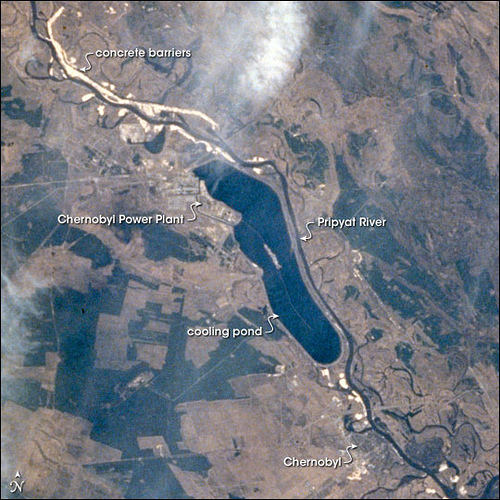
\includegraphics[width=0.5\linewidth]{chernobyl_plant_map}
	\caption{Chernobyl - Map of the plant and colling ponds. The Chernobyl plant and cooling pond are shown in this overhead satellite image captured 10 years after the initial accident}
	\label{fig:chernobylplantmap}
\end{figure}



{\begin{figure}
		\centering
		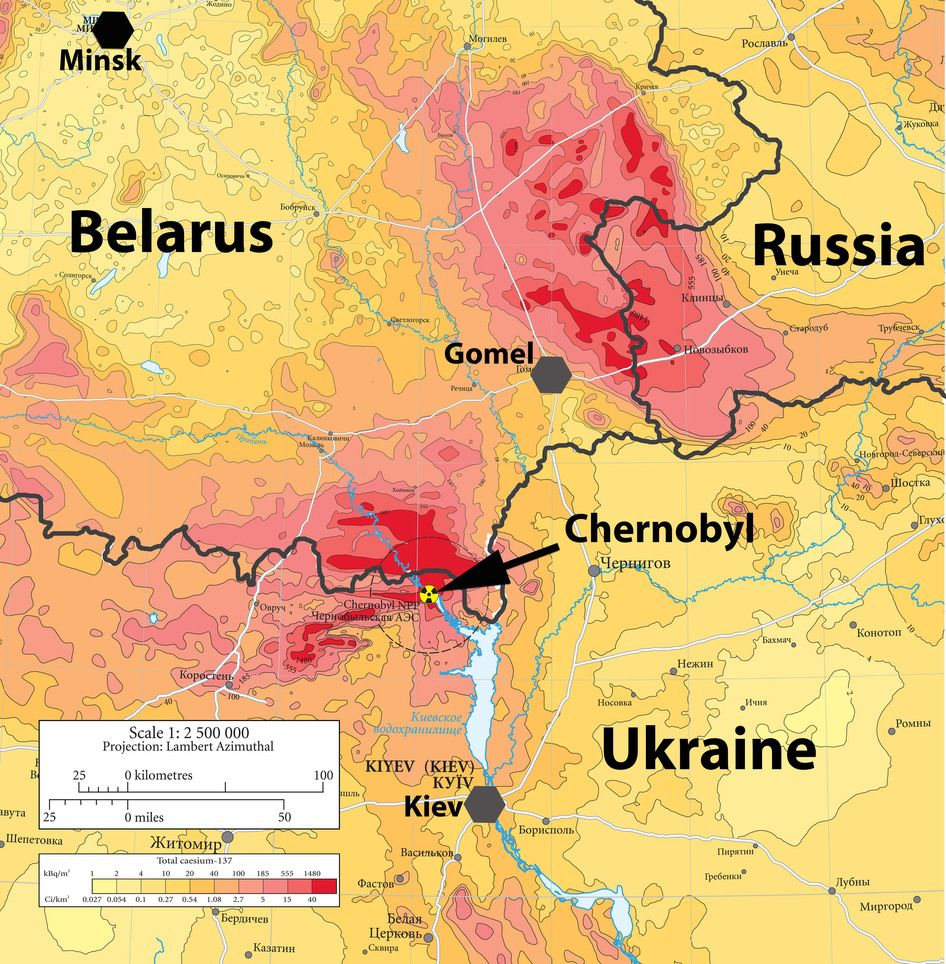
\includegraphics[width=0.5\linewidth]{chernobyl_caesium_137}
		\caption{Chernobyl - Map of caesium-137. The highly radioactive isotope caesium-137 has a medium-term lifespan, with a half-life of around 30 years. However, the damage it causes environmentally is magnified by the ease at which is spreads in the environment due to its water solubility}
		\label{fig:chernobylcaesium137}
	\end{figure}
}{}
\begin{figure}
	\centering
	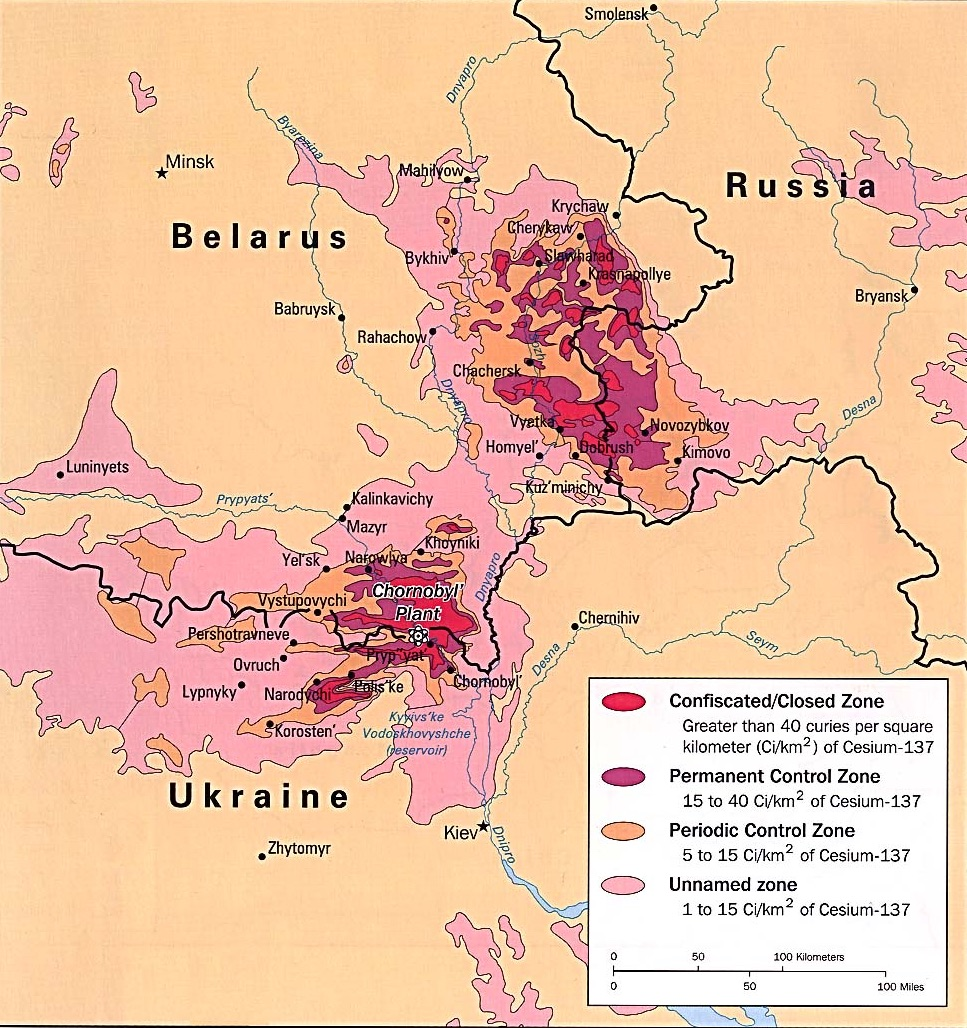
\includegraphics[width=0.5\linewidth]{chernobyl_restricted_zones}
	\caption{Chernobyl - Map of restricted zones - Due to contamination there were exclusion zones set up around the Chernobyl plant over substantial tracts of land in the Ukraine, into Belarus, and affecting as far away as Russia}
	\label{fig:chernobylrestrictedzones}
\end{figure}

\begin{figure}
	\centering
	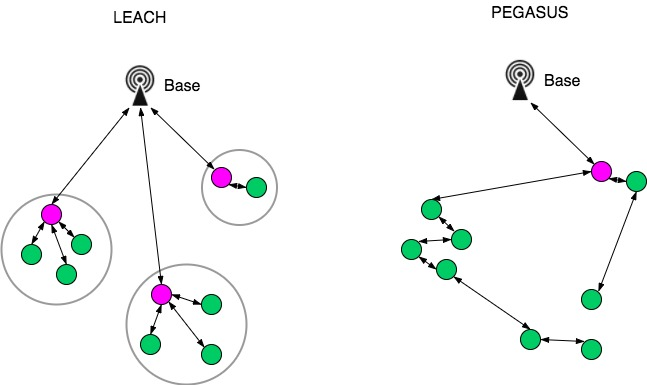
\includegraphics[width=0.7\linewidth]{WSN_simulation_standard_algorithms}
	\caption{WSN standard algorithms - Some standard algorithms for networking in WSN. LEACH uses cluster of nodes each with a lead node for data aggregation and coordination which is rotated periodically to balance power usage. PEGASUS uses chains of nodes with one lead node communicating to the base station.}
	\label{fig:wsnsimulationstandardalgorithms}
\end{figure}

In the event of an incident at a nuclear facility there is a risk that there can be leaks of contaminated radioactive material. This can occur as an atmospheric release or as water that has passed through the cooling system escapes directly into the ground water around the facility instead of being captured in storage ponds for decontamination. In the case of a serious meltdown event such as Chernobyl \cite{Steinhauser2014, Evangeliou2016, Konoplev1992, Fesenko2007, Kortov2013} shown in Figure \ref{fig:chernobylplantmap} we can see a large release of radioactive material into the atmosphere which is then spread globally by winds, contaminating large swathes of the local geographical area, europe, and beyond. We also see this in the many events doumented at the troubled Indian Point plant\cite{TheGuardian} and others where atmospheric releases and ground water contimation have happened repeatedly to varying scales over many years.                                                                                                                                                                                                                                                                                                                                                                                                                                                                                
\newline
\newline


In Chernobyl, lethal levels of radiation were spread over large expanses of remote terrain and have persisted for decades, the land remaining sealed off and uninhabited for over 30 years. These levels mean that humans cannot spend significant time inside the contamination zone without risking rapidly succumbing to the effects of radiation poisoning. Figures \ref{fig:chernobylcaesium137} and \ref{fig:chernobylrestrictedzones} show the contamination areas resulting from the release of the radioactive isotope caesium-137 and corresponding human exclusion zones. Situations like this are unfortunately not that uncommon, although not frequently at such a devastating scale as the Chernobyl or Fukishima disasters. The environmental degradation, essential monitoring characteristics, and harsh external conditions for both humans and machines shown in these cases will prove a fitting and practical testbed for a sensor network deployment based around our agent system.
\newline
\newline


Wide area radioactive contamination gives us a real-world condition that draws out the reasons behind some of the assumptions and criteria used to drive the agent systems learning and operation. In particular, there can be little to no human involvement in deployment or maintenance of sensors deployed to such an environment, the risk to life is simply too large. With this in mind, deployment of sensors is likely to be at-a-distance, and in being so, will have relatively ad-hoc placement. For example, sensors dropped from \textit{Unmanned Aerial Vehicles (UAV)} with no ability to place or move the sensors once released. With a contamination event we may also require sensor readings for many decades, how the adaptation and resilience of an agent-based sensor depoyment can provide for that would prove extremely beneficial to its viability as a solution. Lastly we will see how we can utilise the learning-guided inter-agent linking of the system to give us a robust and resilient networking capability. In addition, dependent on our strategy we can target optimisation of energy utilisation for these low-power remote sensor systems, or should more accurate data be required we can adapt to preferring a greater amount of more granular aggregation of data but at a higher energy cost. 




\subsection{Networking and routing in E-WSN}

In real world deployments it has shown to have been key to balance network robusiness and resilience to damage, alongside the demanding nature of the low energy usage requirements, in order to make the deployments practical, maintainable, and cost-effective. Aside from standard star and peer-to-peer network topologies \cite{Oliveira2011} there have been efforts to develop more targeted architectures based on experience of past WSN \ref{Singh2017, BaniHani, Mahapatra2015, MdZin2014}. Figure \ref{fig:wsnsimulationstandardalgorithms} shows two such algorithms illustrating generalised groupings of these approaches. LEACH uses the idea of sub-clusters of nodes with a nominated lead node that acts as the co-ordintaor and broadcaster of the data back to a base station. These lead nodes are on-hop in that they broadcast directly to the base station, the energy drain caused by this is mitigated by occasionally rotating the lead nodes within the cluster. PEGASUS shows the other main approach to networking with one node acting as the lead node to orchestrate communication with the base station, but there is a multi-hop chain of sub-nodes that relay data through the system using a nearest-neighbour strategy for data request and return. Should a node in the chain go down then the chain will align itself to reform a complete chain back to the base station again. 
\newline
\newline


Comparing these standard algorithms back to the agent system we can see both the similarities with both approaches, but also substantial benefits of the agent-based learning enhancements. The hierarchical approach to agent networking is similar to that we take here, and has been investigated for holoarchy-style agent learning systems such as that of Holmesparker et al \ref{Holmesparker}. The agent system we have set out has both clusters and chains of nodes and clusters as a natural outcome of its operation, with both single-hop and multi-hop both possible outcomes of the structure development through learning links and channels. The networking behaviour is shaped by the definition of local neighbourhood learning for agents and is guided by the higher-level information conveyed by rewards rather than any explicit definitions of networking or agent-system design patterns. While a hierarchical design with lead-agents learning to guide teams of other agents may bear some resemblance to our neighbourhood learning based system, in practice the behaviours within our system are flexible and self-organised to a much greater extent. Scalability itself is incorporated automatically as a direct outcome of placing constraints on neighbourhood formations.
\newline
\newline
\begin{figure}
	\centering
	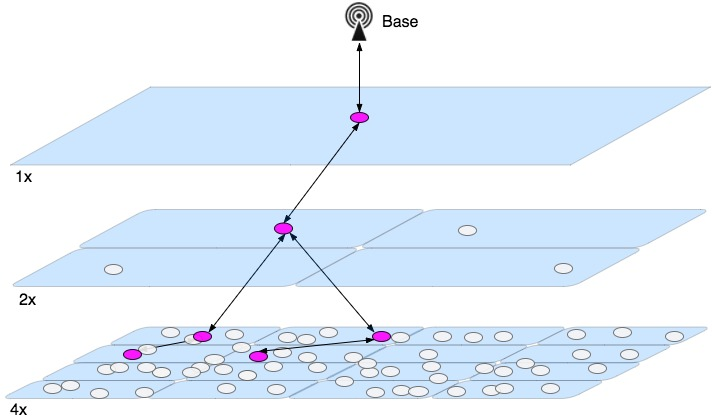
\includegraphics[width=0.7\linewidth]{WSN_hierarchical_resolution}
	\caption{Agent system hierarchical neighbourhood resolution - This diagram shows one of the possible modes of hierarchical networking that can be formed by the agent system through per-agent local neighbourhood learning. The initial agent passes requests through smaller and smaller neighbourhoods until the granulaity of the data meets that of the request}
	\label{fig:wsnhierarchicalresolution}
\end{figure}
\begin{figure}
	\centering
	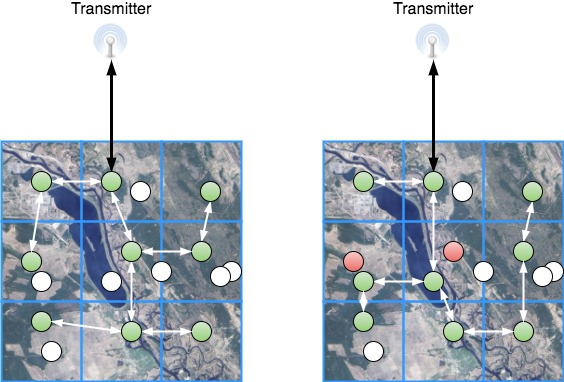
\includegraphics[width=0.7\linewidth]{WSN_simulation_map_failure_adaptation}
	\caption{WSN simulation failure adaptation - The first figure shows a set of agents aggregating data across a defined granularity geographical area using their learned neighbourhoods. In the second we see the adaptation of each agents local neighbourhood as they individually react to device failures}
	\label{fig:wsnsimulationmapfailureadaptation}
\end{figure}

The idea of nearest-neighbour is also applied, but in a more flexible manner and at a higher-level abstraction. While there are definite physical and geographical consequences of deployment such as the range of the transceiver and occlusion behind objects, the agents learn routes with a much wider range of information. Elements such as transfer rate and reliability are large factors in the shape of the reward signals received by agents, but the signal for local neighbourhood formation contains a multitude of other factors and can also be shaped to fit the desired application. So congestion, data consistency, energy cost for transmission and many other factors could be used as elements of the reward heuristic, giving the agents local neighbourhood the shape that best meets with our particular demands on a situational basis. Figure \ref{fig:wsnhierarchicalresolution} illustrates how the agent system works with hierarchical clusters of local neighbourhoods. In reality, the diagram masks the dynamic nature of these neighbourhoods for each agent. Additionally the route through the network of any requests is heavily dependent on the agent that receives an initial request as its neighbourhood will heavily influence the subsequent paths of the requests.
\newline
\newline
With our approach of neighbourhood learning and adaptation for agents we automatically get networking recovery in the event of device failure. Figure \ref{fig:wsn_simulation_failure_adaptation} shows a simplified version of how this might apply when used in agent devices spread over a geographical data, with the grid representing the necessary granularity of the sensor readings. In the first figure, we have an agent aggregating other agent sensor readings as defined by its learned local neighbourhood. We then lose two of the sensors that were on devices that formed the most-optimal data reading request channels in other agents neighbourhoods. The second figure shows how the agents then quickly learn to prioritise data requests over other channels to form an adapted neighbourhood, although this step could also have introduced new channels as part of a state-action space adaptation by the agent to recover connectivity. This shows how we can deploy an agent-system that can adaptively recover from significant outages across the sensor network.


\subsection{Power consumption and recovery}

Another important aspect in the envisaged E-WSN system is the price of inter-agent communication as dictated by the energy consumption of each sensors transceiver while broadcasting. To make the deployment feasible we need a low-energy use system, while still having agents dynamically self-coordintate and using their communication channels to retrieve data readings. With the concept of channels already included within our agent system we can add this easily to the simulation by providing an energy cost to links through these channels. This equates to the power necessary to broadcast throught this communication channel, simulating distance between agents, occlusions, and atmospheric effects that may force higher power requirements on the transeiver if utilised in a real environment. In this way, each message passed through a link will not only shape the subsequent reward through return time, but also through the energy cost of the message. This will ensure that we are not only having agents learn the most efficent data transfer behaviours, but also have the energy efficiency of their requests impact the learning. We also must take in to account the need to spread power distribution across the system. There cannot be a small subset of nodes that are handling the majority of the functionality and therefore the energy usage as their batteries and solar top-up systems will become overwhelmed. Instead we must learn to spread the load, indeed this is exactly what the congestion simulation proviously did through delaying data return times.
\newline
\newline
Now having extended this concept and added an energy consumption measure to agents channels which are proportional to the energy use generated by messages passing through their links, we can use this to accumulate energy consumption rates for those linked-to agents, and use this to drive the requesting agent learning towards adaptation in the face of overloading links. Using $E\textsubscript{cost} $ as the energy cost of making a broadcast request through a link, and $E\textsubscript{rec}$ as the energy recovered by the solar panels of the device per unit of time. We can then use the set of actions on a link $l$ at time $t$ as  $\mathbb{A}_l^t$ to define the actions that cause the link to broadcast, and therefore use energy. We can therefore specify the current energy usage $E\textsubscript{usage} $ of the link as,

\begin{equation}
	E\textsubscript{usage} =  \sum\limits_{i=0}^{t}
	(E\textsubscript{cost} - E_{rec}^{(t-i)})
	\times \mathbb{A}_l^i
\end{equation}
\newline
\newline

We then use the energy usage of a link as a negative factor in our rewards for the requesting agent. Energy costs such as altering links and channels are already encapsulated within the agent system as fixed negative rewards.